\documentclass[10pt,a4paper]{article}
\usepackage[T1]{fontenc}
\usepackage{lmodern}
\usepackage[utf8]{inputenc}
\usepackage[margin=1.8cm,top=1.5cm,bottom=1.5cm]{geometry}
\usepackage{graphicx,booktabs,enumitem,url,caption,titlesec}
\usepackage[colorlinks=true,urlcolor=blue,linkcolor=black]{hyperref}
\captionsetup{font=small,labelsep=none,skip=3pt}
\setlength{\parindent}{0pt}\setlength{\parskip}{3.5pt}
\titleformat{\section}{\large\bfseries}{}{0pt}{}
\titlespacing*{\section}{0pt}{7pt}{3pt}
\setlist{nosep,leftmargin=1.4em,itemsep=2pt}
\pagestyle{empty}
\begin{document}
\begin{center}
{\Large\bfseries TinyCD: spotting changes between two photos with a very small neural network}\\[3pt]
Shresth Keshari \quad|\quad CE712 Mini Project report
\end{center}
\vspace{-4pt}

\section*{1. What is TinyCD?}
\textbf{Change detection} means comparing two photos of the same place taken at different times (for example an aerial photo from 2015 and another from 2020) and marking the pixels where something really changed, such as a new building. The answer is a black-and-white map: white where there is change, black everywhere else.

This is harder than subtracting one photo from the other. Light, season, shadows and small shifts of the camera also change the pixels, but they are not real changes. Real changes are also rare: in the test set we use, only about 5\% of the pixels belong to a change.

Good models for this task are usually big. BIT has about 3 million numbers to learn (its \emph{parameters}) and ChangeFormer about 41 million. \textbf{TinyCD} (Codegoni, Lombardi and Ferrari, \emph{Neural Computing and Applications}, 2023) reports accuracy as good as or better than such models with only \textbf{285,128} parameters. That is about 10 times fewer than BIT and 140 times fewer than ChangeFormer. A small model needs less memory and computing power, which matters when pictures must be processed on cheap or on-board hardware.

\textbf{What we did.} We did not train anything. We wrote the TinyCD network ourselves from the paper, loaded the weights that the authors released, and checked whether it behaves as the paper says. Section 2 explains the model in plain words; Section 3 shows what the replication demonstrates.

\section*{2. How TinyCD works}
\begin{figure}[h!]\centering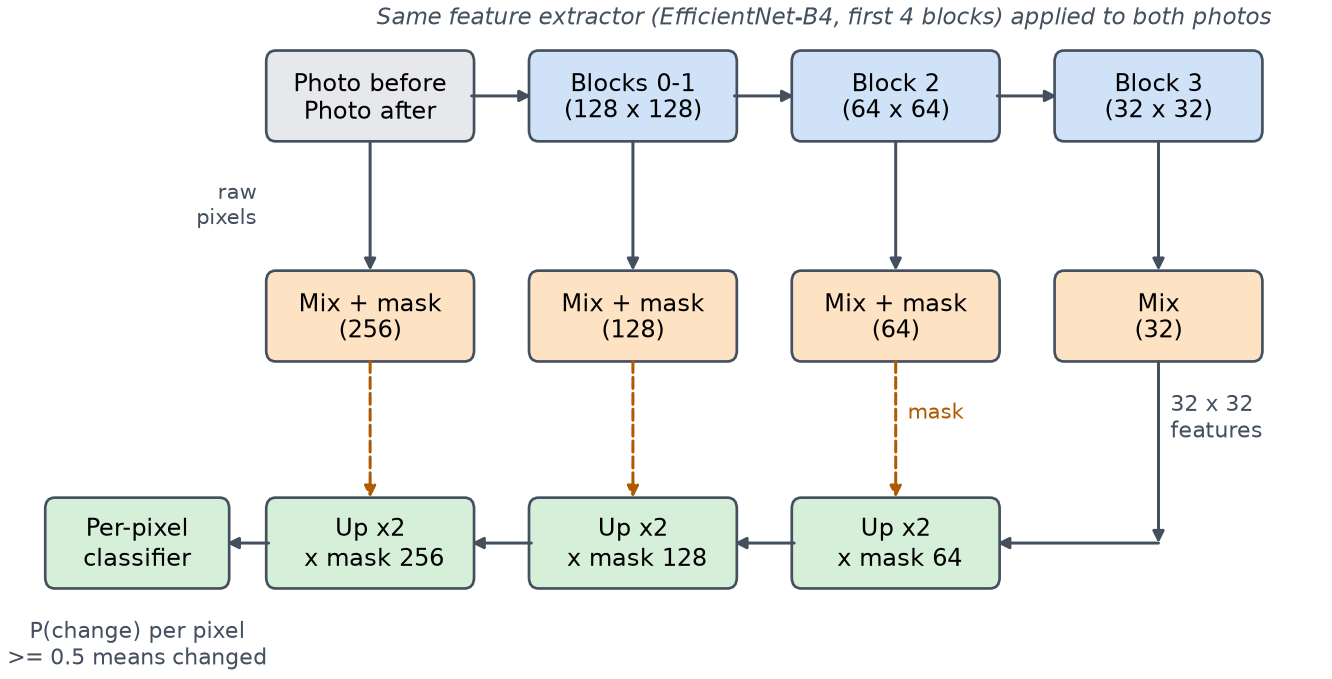
\includegraphics[width=0.92\linewidth]{figures/architecture.png}\caption*{\textbf{Figure 1.} TinyCD. Both photos pass through the same small feature extractor (top row). At each size a \emph{Mix} block compares the ``before'' and ``after'' features (middle row). Three of these also produce a one-number-per-pixel \emph{mask} (dashed arrows) that guides the decoder (bottom row), which grows the picture back to full size.}\end{figure}
The model is a ``U-shaped'' network with four simple ideas:

\begin{enumerate}\item \textbf{One feature extractor for both photos.} Each photo goes through the same network (a ``Siamese'' design), the first four blocks of EfficientNet-B4. It turns the photo into compact maps of edges, textures and shapes at three sizes (128, 64 and 32 pixels wide for a 256-pixel photo). Using the same weights for both photos means a feature means the same thing before and after.
\item \textbf{Mix: a cheap way to compare.} Common ways to compare are to subtract the features or to stack them and apply a large filter. Mix instead interleaves the channels (before-1, after-1, before-2, after-2, and so on) and gives each pair its own tiny filter. Each filter therefore sees one feature as it was before and as it is after, and only has to learn ``did this change?''. This costs very few parameters.
\item \textbf{Masks: tell the decoder where to look.} At full photo size and at the 128 and 64 sizes, Mix is followed by a tiny per-pixel network that outputs one number per pixel: how likely it is that something changed here. The decoder multiplies its own features by these masks, so places that did not change are quieted down.
\item \textbf{A small decoder.} Three steps each double the size, multiply by a mask, and apply a light two-step filter (a depth-wise separable convolution). A last tiny per-pixel network gives the probability of change; we call a pixel changed when it is at least 0.5.
\end{enumerate}
\begin{table}[h!]\centering\small
\begin{tabular}{lrr}
\toprule
Part & Parameters & Share \\
\midrule
Feature extractor (EfficientNet-B4 blocks 0-3) & 269,362 & 94.5\% \\
Mix and masks (4 scales) & 3,357 & 1.2\% \\
Decoder (3 Up blocks) & 11,734 & 4.1\% \\
Per-pixel classifier & 675 & 0.2\% \\
\textbf{Total} & \textbf{285,128} & \textbf{100\%} \\
\bottomrule
\end{tabular}
\caption*{\textbf{Table 1.} Where TinyCD's parameters are (counted from our implementation). The parts that do the comparing (Mix, masks, classifier) hold only 4,032 parameters, 1.4\% of the model.}\end{table}
\section*{3. What the replication shows}
We evaluated on \textbf{LEVIR-CD}: 2,048 test pairs of 256 $\times$ 256 aerial photos (0.5 m per pixel) in which people marked new or demolished buildings. Every model used the same 0.5 threshold and the weights released by its authors. BIT and ChangeFormer were run with their official code for comparison. Each point below is a claim we checked.

\textbf{(a) Our network is the authors' network.} The released weights load into our code with strict matching: every name and shape agrees, and the total is 285,128 parameters, as in the paper. We also rebuilt the paper's variants (Mix replaced by subtraction or by stacking, no final classifier): the full model, seven variants and the B3 backbone match the paper's counts exactly. The B0, B1 and B2 backbones differ from the paper by 272 parameters (about 0.2\%); we did not find the cause.

\begin{table}[h!]\centering\small
\begin{tabular}{lrr}
\toprule
Variant & Our count & Paper \\
\midrule
Full TinyCD & 285,128 & 285,128 \\
Mix replaced by subtraction (everywhere) & 282,939 & 282,939 \\
Mix replaced by stacking + filter (everywhere) & 368,468 & 368,468 \\
No final classifier & 282,438 & 282,438 \\
Backbone B3 (instead of B4) & 178,716 & 178,716 \\
Backbone B2 & 147,768 & 148,040 \\
Backbone B1 & 121,820 & 122,092 \\
Backbone B0 & 79,208 & 79,480 \\
\bottomrule
\end{tabular}
\caption*{\textbf{Table 2.} Parameter counts of the paper's variants, rebuilt by us (a selection of the 13 we checked). Only the full model has released weights, so only counts, not accuracies, are compared.}\end{table}
\textbf{(b) The accuracy is as reported.} \emph{F1} is one score from 0 to 100 that rewards finding real changes and not raising false alarms. TinyCD scores 91.07, against 91.05 in the paper (Table 3). ChangeFormer matches its paper (90.40). BIT scores 89.94, higher than the 89.31 it reports; we do not know why and report it as measured. To see whether TinyCD's lead is real, we resampled the test images 2,000 times: it is ahead of BIT by 1.12 points (95\% interval 0.69 to 1.57) and ahead of ChangeFormer by 0.67 (0.29 to 1.00). So TinyCD is at least as accurate here, but not dramatically better; the point is the same accuracy at a tiny size.

\begin{table}[h!]\centering\small
\begin{tabular}{lrrrrr}
\toprule
Model & F1 \% (95\% interval) & Paper F1 & Parameters & GFLOPs & CPU s / pair \\
\midrule
\textbf{TinyCD} & \textbf{91.07} (90.63-91.45) & 91.05 & \textbf{285,128} & \textbf{1.46} & \textbf{0.19} \\
BIT & 89.94 (89.35-90.53) & 89.31 & 3,037,026 & 8.76 & 0.27 \\
ChangeFormer V6 & 90.40 (89.82-90.93) & 90.40 & 41,026,674 & 138.80 & 2.45 \\
\bottomrule
\end{tabular}
\caption*{\textbf{Table 3.} LEVIR-CD test set (2,048 pairs), threshold 0.5, released weights. GFLOPs: billions of operations for one 256 $\times$ 256 pair. CPU time: median for one pair on our laptop (batch of 1). BIT's checkpoint holds 11.9 M numbers; 3.04 M are used at test time.}\end{table}
\textbf{(c) It is much cheaper to run.} TinyCD needs 1.46 billion operations per pair, against 8.76 for BIT and 138.8 for ChangeFormer. On our laptop CPU it takes 0.19 s per pair, against 0.27 s and 2.45 s. (BIT is only 1.4 times slower despite 6 times more operations: running time depends on more than the operation count.)

\clearpage
\textbf{(d) We can see it work, and fail.} Figure 2 shows TinyCD finding a large and a small new building. It also shows a miss and a false alarm. Over the whole test set it finds 89.2\% of the 8,673 separate changed regions (BIT 88.4\%, ChangeFormer 88.7\%).

\begin{figure}[h!]\centering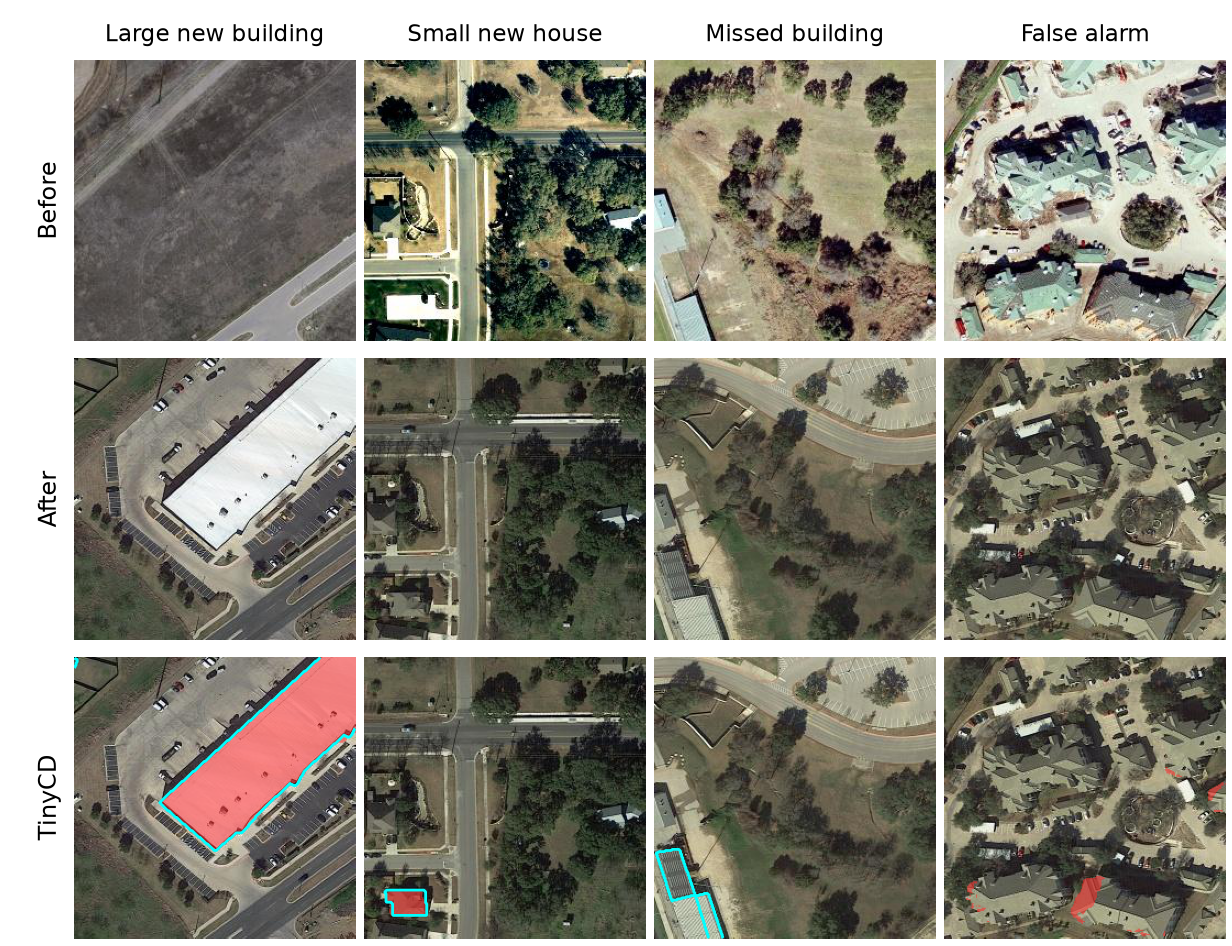
\includegraphics[width=0.86\linewidth]{figures/qualitative.png}\caption*{\textbf{Figure 2.} Four test pairs (before, after, and TinyCD's answer in red; the human label is outlined in cyan). Left to right: a large new building, a small new house, a building TinyCD misses, and a false alarm on roofs that did not change.}\end{figure}
\textbf{(e) The masks matter.} As a probe, we switched off one mask at a time in the released model (by setting it to 1). Without the 64-size mask, F1 falls to 82.1; without the 128-size mask, to 90.1; without the full-size mask, to 0.3. This shows the trained network depends on its masks. It is not a retrained ablation, so it does not show how a network trained without masks would do.

\textbf{What we did not show.} We did no training, so the paper's ablation accuracies and results on other datasets are not re-measured. TinyCD was trained on 0.5 m building changes; it should not be expected to work on very different resolutions or satellites. All timings are from one laptop.

\section*{4. Summary}
\begin{itemize}\item TinyCD is small because it keeps only the first four blocks of a compact feature extractor and does the comparing with very cheap blocks (Mix and masks).
\item With the authors' weights, our implementation reproduces the reported accuracy on LEVIR-CD (F1 91.07 against 91.05) with about 10 times fewer parameters than BIT and 140 times fewer than ChangeFormer, and about 6 and 95 times fewer operations.
\item It is not perfect (it misses some buildings and raises some false alarms), and our checks cover one dataset and no retraining.
\end{itemize}
\textbf{Try it.} Live demo in the browser (no install): \url{https://shresth-keshari.github.io/tinycd-demo/}. Code, Colab notebook and a one-step run script: \url{https://github.com/shresth-keshari/tinycd-demo}. The demo runs the real TinyCD model on sample pairs or on your own pair of photos.

\end{document}